\documentclass[sigplan,screen]{acmart}
\usepackage{graphicx}

%%
%% \BibTeX command to typeset BibTeX logo in the docs
\AtBeginDocument{%
  \providecommand\BibTeX{{%
    \normalfont B\kern-0.5em{\scshape i\kern-0.25em b}\kern-0.8em\TeX}}}

%% Rights management information.  This information is sent to you % when you
%complete the rights form.  These commands have SAMPLE % values in them; it is
%your responsibility as an author to replace % the commands and values with
%those provided to you when you % complete the rights form.
\setcopyright{acmcopyright}
\copyrightyear{2018}
\acmYear{2018} \acmDOI{10.1145/1122445.1122456}

%% These commands are for a PROCEEDINGS abstract or paper.
% \acmConference[Woodstock '18]{Woodstock '18: ACM Symposium on Neural Gaze
% Detection}{June 03--05, 2018}{Woodstock, NY} \acmBooktitle{Woodstock '18: ACM
% Symposium on Neural Gaze Detection, June 03--05, 2018, Woodstock, NY}
% \acmPrice{15.00} \acmISBN{978-1-4503-XXXX-X/18/06}

%%
%% Submission ID. % Use this when submitting an article to a sponsored event.
%You'll % receive a unique submission ID from the organizers % of the event, and
%this ID should be used as the parameter to this command.
%%\acmSubmissionID{123-A56-BU3}

%%
%% end of the preamble, start of the body of the document source.
\begin{document}
\title{Improved Macroscopic Traffic Flow Modelling with Cellular Automata}

%%
%% The "author" command and its associated commands are used to define % the
%authors and their affiliations. % Of note is the shared affiliation of the
%first two authors, and the % "authornote" and "authornotemark" commands % used
%to denote shared contribution to the research.
\author{Noah Gardner}
\authornote{All authors contributed equally to this research.}
\email{ngardn10@students.kennesaw.edu}
\orcid{0000-0001-5900-9841}
\affiliation{%
    \institution{College of Computing and Software Engineering }
    \streetaddress{1100 South Marietta}
    \city{Marietta}
    \state{Georgia}
    \country{USA}
    \postcode{30060}
}

\author{Andy Vu}
\authornotemark[1]
\email{avu5@students.kennesaw.edu}
\affiliation{%
    \institution{College of Computing and Software Engineering }
    \streetaddress{1100 South Marietta}
    \city{Marietta}
    \state{Georgia}
    \country{USA}
    \postcode{30060}
}

\author{Olivier Tran}
\authornotemark[1]
\email{otran@students.kennesaw.edu}
\affiliation{%
    \institution{College of Computing and Software Engineering }
    \streetaddress{1100 South Marietta}
    \city{Marietta}
    \state{Georgia}
    \country{USA}
    \postcode{30060}
}

\author{Sanjeev Khemani}
\authornotemark[1]
\email{skheman1@students.kennesaw.edu}
\affiliation{%
    \institution{College of Computing and Software Engineering }
    \streetaddress{1100 South Marietta}
    \city{Marietta}
    \state{Georgia}
    \country{USA}
    \postcode{30060}
}

%%
%% By default, the full list of authors will be used in the page % headers.
%Often, this list is too long, and will overlap % other information printed in
%the page headers. This command allows % the author to define a more concise
%list % of authors' names for this purpose.
\renewcommand{\shortauthors}{Gardner et al.}

%%
%% The abstract is a short summary of the work to be presented in the % article.
\begin{abstract}
    This paper is based on another research paper in cellular automata in which
    city traffic and its affection by factors such as distributed occurrence,
    evanescence, and time variation is observed on a two-dimensional grid. The
    variables used in this new experiment include diagonal paths, one-way
    streets, pre-generated flows, varying speeds, varying destination priority,
    and different types of roads. With these additional factors in the
    experiment, the results of the new simulation may yield results that more
    accurately reflect the environment of real-world traffic.
\end{abstract}

%%
%% Keywords. The author(s) should pick words that accurately describe % the work
%being presented. Separate the keywords with commas.
\keywords{traffic flow, cellular automata}

%%
%% This command processes the author and affiliation and title % information and
%builds the first part of the formatted document.
\maketitle

\section{Research Statement}
There are a few interesting changes we could make to the original algorithm in
order to explore the impact of different traffic environments and flows. For
example, the original paper randomly generates \textit{traffic flows} which are
an abstracted representation of the traffic that actually represents a group of
vehicles as a random amount of traffic. Additionally, when each traffic flow is
generated, the destination of the flow is also generated randomly. After the
traffic flow is generated and the destination is chosen, the traffic flow
chooses it's path automatically as the shortest distance from the starting cell
to the current cell. Finally, the original paper uses one traffic environment
with simple two-way roads that are placed on the grid laterally and vertically.

One idea we would like to explore is to add different priorities for cells as
destinations. If a cell is a high priority destination, then it is more likely
to be chosen as a destination for a traffic flow when it is generated. Another
improvement could also allow for modelling of different types of roads. For
example, rather than the flow taking the shortest path from the source to the
destination, each cell could have a parameter for the weight of adding that cell
to the path of the traffic flow. If the weight of adding the cell to the path is
low, that cell may be modeled as part of a road that can handle more traffic
such as a highway. The original experiment also did not test diagonal or one-way
streets, so that may be valuable for a traffic flow model as well.

\section{Related Works}
% Simulation of urban macro-traffic flow based on cellular automata
          
Authors et al. use a cellular automata model to simulate traffic flow on a
two-dimensional grid \cite{pang_simulation_2019}. Traffic flows are randomly
generated that have a certain amount of traffic (low or heavy) and also have a
random destination. There exists a grid with cells filled in which are meant to
model the roads for the traffic flow to move on. On each timestep, the traffic
flows move towards their destination using a minimum distance method. The cells
can hold a certain amount of traffic capacity. When the traffic capacity for a
cell is reached, the cell will not allow new traffic flows to enter the cell.
The cells also have a traffic volume, which helps the programmer to see at a
glance which cells have high and low volumes of traffic.

% A cellular automaton model for freeway traffic
          
Nagel and Schreckenberg have gone away from the typical fluid dynamical
approaches to traffic flow studies during this time to the use of a more
revolutionary technique \cite{nagel_cellular_1992}. The need for this was to
introduce a factor of laminar start-stop waves with increasing vehicle density
with an emphasis on human behavior a traffic environment. In their model, it is
represented as a single dimensional array where each cell may be a vehicle with
functions to accelerate, slow down, as well as randomized velocities. These
functions are to represent the randomness in human behavior and varying
conditions that are expected during traffic. The authors concluded that a
computational way to simulate traffic flow, was more advantagous to a fluid
dynamical approach that incorporated real world behavior of a driver but also
retained the key aspects of fluid dynamic studies.

% Self-organization and phase transition in traffic-flow model of a two-lane
% roadway 

Nagatani implements a two lane model as an extension of a one dimensional
cellular automaton to monitor lane changing.
\cite{nagatani_self-organization_1993} Their model is essentially two
1-dimensional lattices to represent a two lane roadway. Rules using arrows
within the lattice were deteremined to allow cars to change lanes at certain
times such as when a car in front was blocking the path to progress forward from
either the right to left direction or vice versa. These rules were dependent on
the time step. Overall the results showed that as the cars general velocity
increased, there was a usage of lane shifting without cars obstructing progress.
As density increases, the maximal velocity decreases. There was a "sweet-spot"
indicating the optimal amount of lane changing within a set of density of
traffic where lane changing peaked with a critical value of density. If the
density fell or rose too high, this optimal amount of lane changing dropped.


% Multi-value cellular automata model for mixed bicycle flow

Instead of car and vehicle traffic like the other papers, this paper focused on
mixed bicycle flow using a multi valued cellular automata.
\cite{jia_multi-value_2007} Here the authors implemented two bicycles with
different maximum speeds. The usage of bicycles to compare to vehicles have an
emphasis on the behavioral and personality aspect that can be difficult to
analyze with cars. The authors explain that young riders tend to ride at high
speeds while older riders ride at a lower speed. These differences show that
there is no set maxium velocity. In this model, bicycles can move to their next
open site with faster bicycles moving with priority over slower bicycles. It was
shown similarily to vehicles that slow bicycles that congregate and occupy
sites, block faster moving bicycles that cannot overtake and thus move in a
platoon order. Increasing slow bicycle density will congest and bottleneck the
simulation. One of the points that B. Jia and the authors mention that cannot be
properly analysed is the nature of riders that group together because they are
classmates or friends thus this simulation does have some flaws. Increasing
randomization of the locations and density of slow riders tended to allow more
free flow and less bottlenecking.


% Cellular automaton model for bidirectional traffic

Simon and Gutowitz have built upon the paper referenced above by Nagel and
Schreckenberg. \cite{simon_cellular_1998-1} Here they are implementing a
bidrectional traffic using a two lane road with traffic moving in opposite
direction in comparison to Nagel and Schreckenberg's one lane cellular
automaton. They have incorporated inteteractions to simulate passing, as well as
a distribution of varying vehicle speeds. Once again, Simon and gutowitz, like
their reference model, had an emphasis on approximating the behavior of real
traffic and human behavior. They wanted to address the issue of a one lane
cellular atomaton where all vehicles have a maximum velocity and thus the model
unrealistically follows a lead slow car, hence the need and emphasis on passing.
The bidirectional model varried in types where there was varrying rules
regarding passing. The researchers have found that passing greatly increases
fluidity in traffic not seen in single dimensional cellular automaton and
greatly resembles real world traffic dynamics and flow.
          


% A high-resolution celluar automata traffic simulation model with application
% in a freeway traffic information system

Hafstein uses cellular automata to visualize and simulate real word traffic
conditions using inputs that are detected from the North Rhine-Westphalia area
in Germany. \cite{hafstein_high-resolution_2004} Loop detectors are inductive
electrical devices that are put into the road which can record vehicles that are
either passing or sitting upon them. By utilizing these detectors, Hafstein and
others were able to determine the vehicle type, such as truck or car, the
average velocity of these vehicles, and the amount that passed the loop detector
within a time window. Once this data is collected, the data is input into a
high-resolution cellular automaton traffic simulator. Hafstein’s goal was to
improve Nagel’s simulation design with such improvements such as whether a
vehicle should brake or not depending on the distance to the vehicle in the
front. By using a smaller cell and higher density, it allowed more realistic
acceleration and speed bins compared to using larger cells of that in other
simulations. Lastly, regarding the output of the simulation, a graphical 3D
interface was designed to allow city planners to visualize and plan construction
around the highway.

\section{Methods}
For this project, we are using Python to implement our cellular automata traffic
flow model. We also included a simple GUI to visualize the traffic flow on each
time step. Some of the libaries that we are using include: Matplotlib, Seaborn,
Pillow, and Numpy

\section{Progress}

% \begin{figure}
%     \centering
%     \includegraphics{assets/cells.png}
%     \caption{An example of two traffic cells inside the traffic matrix.}
%     \label{fig:cells}
% \end{figure}

% \begin{figure*}
%     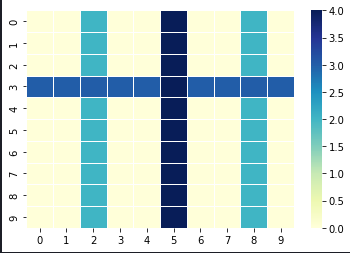
\includegraphics{assets/cmatrix.png}
%     \caption{An example traffic grid.}
%     \label{fig:cmatrix}
% \end{figure*}

% \begin{figure}
%     \centering
%     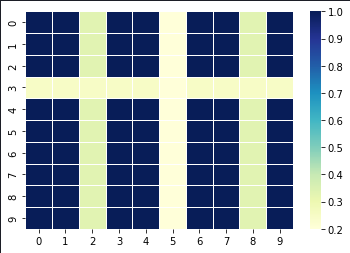
\includegraphics{assets/wmatrix.png}
%     \caption{An example traffic grid, showing the weighted matrix.}
%     \label{fig:wmatrix}
% \end{figure}

As of now at this middle update, we have successfully implemented the original
algorithm. Our matrix road network is different from the original paper. Instead
of an outside loop, with several intersections, our implementation so far is a
simple three vertical paths, with one horizontal path (Fig. \ref{fig:cmatrix}).
With this we have generated cells of varying capacity and density which traverse
stepping through possible moves through the matrix to reach their randomized
terminal destination where from here the cells are removed from system. We can
expand the matrix to any size with any number of starting instances of traffic
flows, however, so far, we have worked with a 10 x 10 matrix for simplicity. 

On top of this, we have also implemented our first step in branching from the
original paper. Here we have developed a weighting system that adds weights to
cells.  By introducing weights to the cells, we able to coerce the traffic cells
to take different routes other than the shortest possible path. We are able to
see if the route of taking a lower weighted route such as a longer highway with
a high traffic capacity would be quicker than a shorter path that allows less
traffic flow with a smaller capacity value. Since the weight is simply the
inverse of the capacity of the cell we can find an optimal path to the
destination. On top of this, we have designed a simple gif to illustrate the
traffic flows in addition to an output that shows corresponding coordinates that
show past and future moves to allow us to better understand the direction and
flow of these cells. This GUI heatmap allowed us to see an intentional design
choice in the original paper that is further discussed in the results section.  

Regarding the destination priorities that was included in our initial project
proposal as a brainstorming idea to branch from the original paper, we have
decided to omit the development of it. We had decided that it would not create
much of an impact in the simulation in terms of priority along the development
timeline. Addressing the weights and their respective functions came as a
priority in addition to the issue found with cells getting stuck without a
circular outside edge path of the matrix.  

Some of the issues that we have run into is the use of technology such as
python, visual studio code and github with several of the group members. This
presents a challenge as there is a disparity in some of these skills between
members. However, despite this, our members are continuously eager to learn and
teach one another. In addition to this, members contribute to their strengths
while others cover their weaknesses. With this, there has been a constant amount
of communication from each member and harmonious work ethic that each member
brings to the table to accomplish the task at hand. Through this mutual
cooperation, we have been able to steadily progress through our milestones.  

\section{Preliminary Results and Analyses}
From our implementation of the original algorithm, we are able to visualize the
flow of traffic. Depending on the number of instances of traffic cells
generated, we can see that the cells are able to move to their destination
within the shortest path given the traffic capacity is accommodating. It is
interesting to see how a cell can quickly reach a high density of traffic once
multiple flows of traffic converge at that matrix coordinate. In addition to
this, it seems that in the original paper, an outer lying circular route at the
edge of the matrix was included to accommodate to the rules of the traffic flow.
Without the outer route, it would be more cost effective for a cell to stay in
its position than to backtrack into another route. By implementing a circular
route along the edges of the matrix, the cells are able to continuously move in
their desired direction to reach the final destination.  

\section{Conclusion and Future Work}
We would like to implement a cost-effective route decision that takes accuracy
as the highest priority to prevent the likely hood of a cell staying in single
position that was discussed in the results section. By implementing this design,
we would be able to have cells reach their destination no matter the cost of the
route, without the use of circular route along the edges of the matrix. This was
a decision we had come up with that presented itself as an issue not foreseen in
the initial project proposal. In addition to this, we are still projected to
model different traffic environments such as one-way streets and further do a
deeper analysis on the traffic simulation model. Most likely an improvement to
the matrix to represent a real-world model would greatly reflect the accuracy of
the simulation. A local road or area where we could compare it with traffic from
another source, we be a great test comparison. Lastly, with time permitting we
would like to further polish our GUI to better visualize the traffic flow
simulation than already accomplished.  

\bibliographystyle{ACM-Reference-Format}
\bibliography{report}

\end{document}
\endinput
